\section{Results}
\label{sec:results}

\subsection{Error Decomposition}
\label{sec:error_decomp}

\Cref{tab:error_decomp,fig:error_breakdown} report the premise/reasoning breakdown
for incorrect answers under Qwen2.5-VL on GQA ($n{=}500$). Of 204 incorrect answers,
\textbf{68 (33.3\%)} involve at least one verifiably contradicted belief, constituting
\emph{premise errors}. The remaining 136 (66.7\%) are reasoning errors. Mean belief
coverage over scene-graph facts is 0.49 (see \cref{fig:claim_coverage}), so the
33.3\% figure is a \emph{conservative lower bound}.
Qwen2.5-VL externalizes an average of 4.96 beliefs per question, enabling substantially
higher premise-error detection than LLaVA-1.5 (2.17 beliefs; 18.8\% PE rate).

\begin{table}[h]
\centering
\caption{Error decomposition by question type (Qwen2.5-VL, GQA, $n{=}500$).
Premise errors are most prevalent in logical/relational questions.}
\label{tab:error_decomp}
\small
\setlength{\tabcolsep}{5pt}
\begin{tabular}{lcc}
\toprule
\textbf{Question Type} & \textbf{Premise Error} & \textbf{Reasoning Error} \\
\midrule
logical  & 50.0\% & 50.0\% \\
compare  & 40.0\% & 60.0\% \\
query    & 32.9\% & 67.1\% \\
verify   & 30.4\% & 69.6\% \\
choose   & 14.3\% & 85.7\% \\
\midrule
\textbf{Overall} & \textbf{33.3\%} & \textbf{66.7\%} \\
\bottomrule
\end{tabular}
\end{table}

\begin{figure}[t]
  \centering
  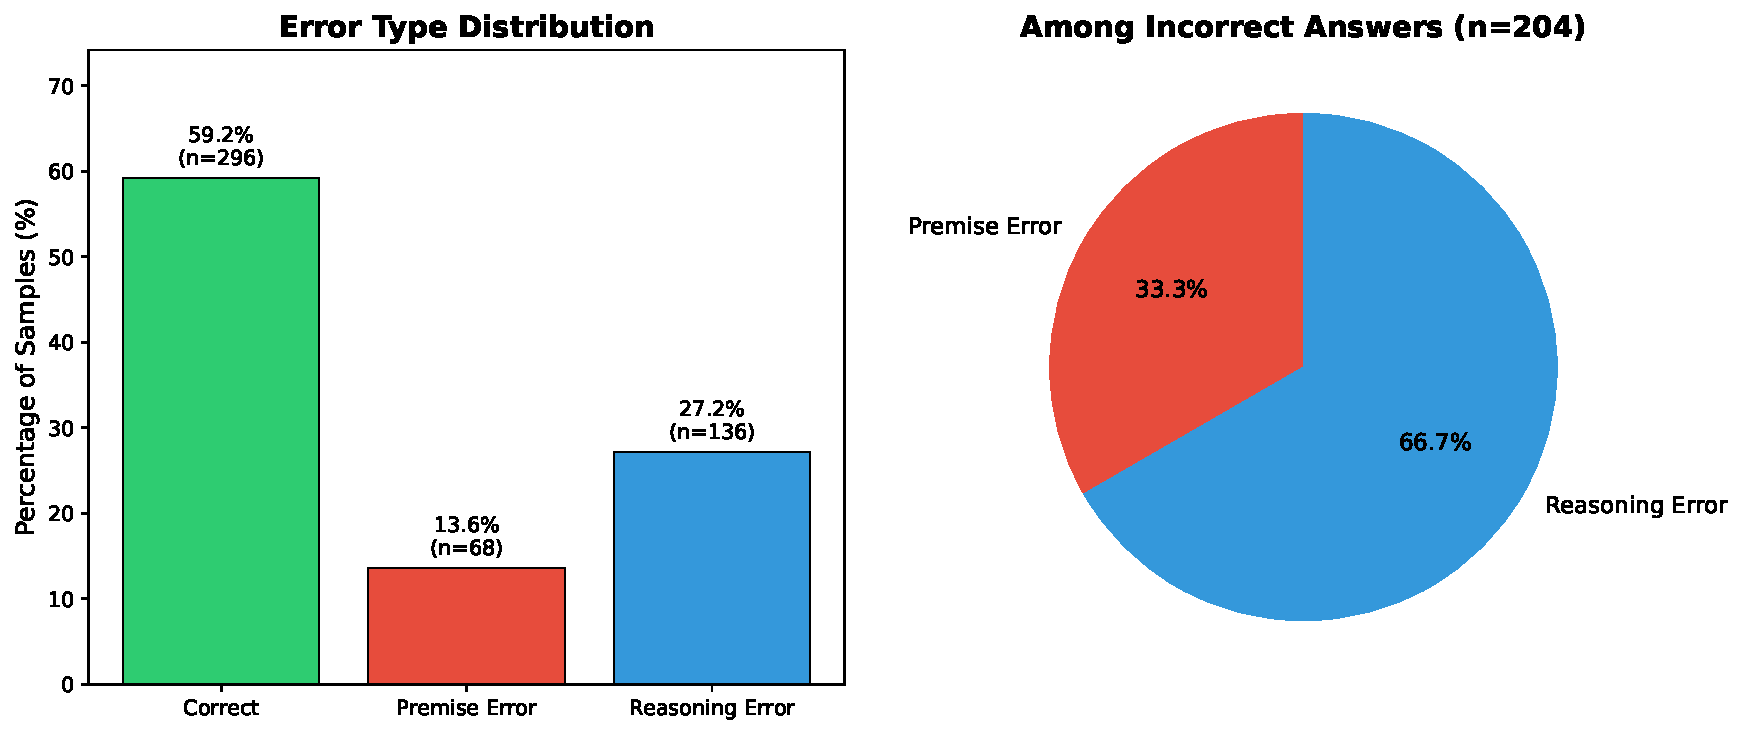
\includegraphics[width=\linewidth]{figures/error_breakdown}
  \caption{Error type distribution for Qwen2.5-VL on GQA ($n{=}500$).
  Left: overall breakdown (59.2\% correct, 13.6\% PE, 27.2\% RE).
  Right: among incorrect answers, 33.3\% are premise errors---a conservative
  lower bound given 49\% mean claim coverage.}
  \label{fig:error_breakdown}
\end{figure}

\subsection{Intervention Results}
\label{sec:intervention}

\Cref{tab:main_results} summarizes all intervention methods at both scales.
\textbf{BCI-E1} achieves the largest gain at $n{=}500$: $+18.0$~pp ($59.2\%
\to 77.2\%$), with 117 samples flipped to correct and only 27 regressed
(McNemar $p{=}1.5{\times}10^{-14}$). \Cref{fig:premise_correction} shows
that among the 68 premise-error cases, correcting false beliefs directly
recovers the correct answer in 60.3\% of them. At $n{=}2000$, E1 achieves $+16.2$~pp
($63.55\% \to 79.75\%$; $p{=}1.78{\times}10^{-48}$) with a flip-to-correct
rate of 21.2\%, confirming that the causal signal scales robustly.

\textbf{BCI-E3} shows near-zero net gain at $n{=}500$ ($-0.6$~pp, $p{=}0.84$),
establishing that \emph{removal alone is insufficient}---replacing false beliefs
with ground-truth facts is the operative mechanism.

\textbf{BCI-E12b} achieves $+3.45$~pp at $n{=}2000$ ($p{=}1.3{\times}10^{-5}$)
while intervening on 59.85\% of samples. Multi-seed evaluation (seeds 42, 123, 456)
yields $66.18\% \pm 0.14$~pp, confirming numerical robustness.

\begin{table}[h]
\centering
\caption{Main intervention results on GQA. BCI-E1 is the causal upper bound;
E12b is the practical bounded-intervention policy.
McNemar exact $p$-values are against the Vanilla baseline.
F$\uparrow$: flip-to-correct rate; F$\downarrow$: flip-to-wrong rate.}
\label{tab:main_results}
\small
\setlength{\tabcolsep}{2.5pt}
\begin{tabular}{lrrrcc}
\toprule
\textbf{Method} & $n$ & \textbf{Acc.} & $\boldsymbol{\Delta}$\textbf{Acc.}
  & \textbf{F$\uparrow$} & \textbf{F$\downarrow$} \\
\midrule
Vanilla        & 500  & 59.2\% & ---        & ---    & ---  \\
Self-Correct   & 500  & 49.2\% & $-10.0$ pp & ---    & ---  \\
CoVe-Lite      & 500  & 57.2\% & $-2.0$ pp  & ---    & ---  \\
Resample-Lite  & 500  & 60.6\% & $+1.4$ pp  & ---    & ---  \\
BCI-E3         & 500  & 58.6\% & $-0.6$ pp  & 9.4\%  & 10.0\% \\
\textbf{BCI-E1}& 500  & \textbf{77.2\%} & $\mathbf{+18.0}$ \textbf{pp}
                                          & \textbf{23.4\%} & 5.4\% \\
\midrule
Vanilla        & 2000 & 63.55\% & ---       & ---    & ---  \\
BCI-E12b       & 2000 & 66.35\% & $+2.8$ pp & 7.9\%  & --- \\
BCI-E12b (tuned) & 2000 & 66.35\% & $+3.45$ pp & 7.9\% & --- \\
\textbf{BCI-E1}& 2000 & \textbf{79.75\%} & $\mathbf{+16.2}$ \textbf{pp}
                                          & \textbf{21.2\%} & ---  \\
\bottomrule
\end{tabular}
\end{table}

\begin{figure}[t]
  \centering
  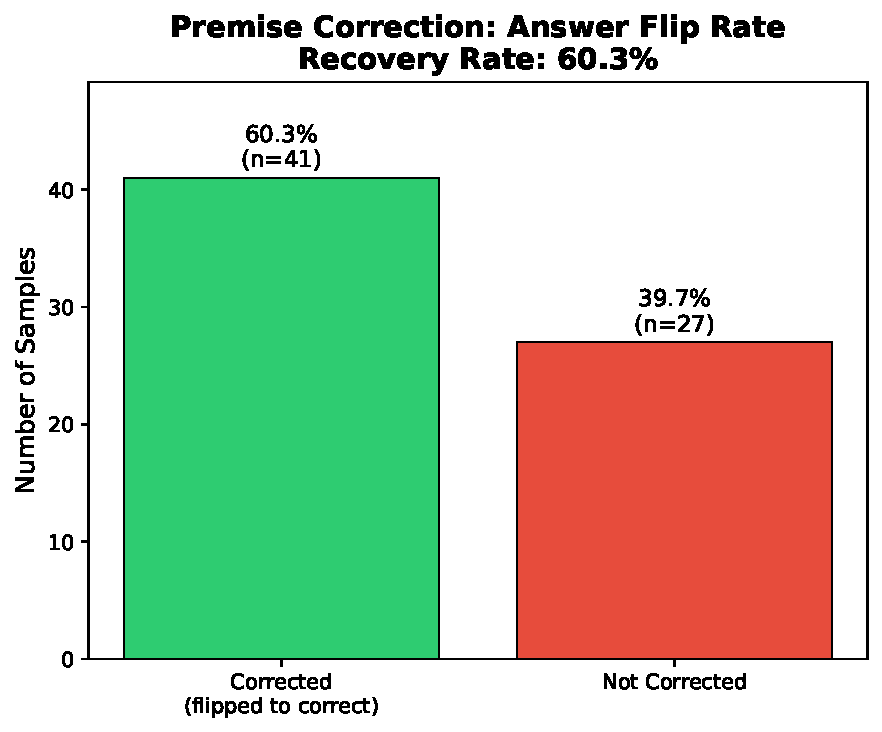
\includegraphics[width=0.75\linewidth]{figures/premise_correction}
  \caption{Premise correction recovery rate among premise-error cases ($n{=}68$).
  Correcting contradicted beliefs flips 60.3\% (41/68) of premise-error cases
  to the correct answer, confirming that false visual premises are the direct
  causal driver in the majority of these failures.}
  \label{fig:premise_correction}
\end{figure}

\subsection{Question-Type Stratification}
\label{sec:stratified}

\Cref{tab:stratified} breaks down E1 and E12b gains by question type at $n{=}2000$.
E1 delivers the largest absolute gains for query-type questions ($+25.9$~pp;
flip-to-correct 29.8\%) and other-type questions ($+20.3$~pp; flip-to-correct 24.3\%).
Verify-type questions, which have high baseline accuracy (80.4\%), show smaller but
still meaningful gains ($+5.6$~pp). E12b shows a similar pattern but with attenuated
gains, particularly for verify ($+0.35$~pp), reflecting the higher difficulty of
identifying high-confidence contradictions in short yes/no-style questions.

\begin{table}[h]
\centering
\caption{Stratified gains by question type (GQA, $n{=}2000$). E1 and E12b
flip-to-correct rates reveal where premise correction is most effective.}
\label{tab:stratified}
\small
\setlength{\tabcolsep}{2pt}
\begin{tabular}{lrrrr}
\toprule
\textbf{Type} & $n$ & \textbf{Base} &
  \textbf{E1 $\Delta$} & \textbf{E12b $\Delta$} \\
\midrule
query    & 887  & 47.0\% & $+25.9$ pp & $+6.2$ pp \\
verify   & 854  & 80.4\% & $+5.6$ pp  & $+0.4$ pp \\
logical  & 57   & 75.4\% & $+8.8$ pp  & $+7.0$ pp \\
other    & 202  & 61.4\% & $+20.3$ pp & $+3.5$ pp \\
\bottomrule
\end{tabular}
\end{table}

\Cref{fig:stratified_structural,fig:stratified_semantic} further decompose these
gains. Among structural question types, E1 most strongly advantages query-type
($+17.0$~pp gap over E12b) and choose-type ($+9.1$~pp gap) questions.
Among semantic sub-types, categorical (``cat'') questions show the largest
E1 advantage ($+20.97$~pp gap), followed by relational questions ($+17.30$~pp),
confirming that premise correction is especially impactful when the answer
depends on identifying object categories and spatial/relational facts.

\begin{figure}[t]
  \centering
  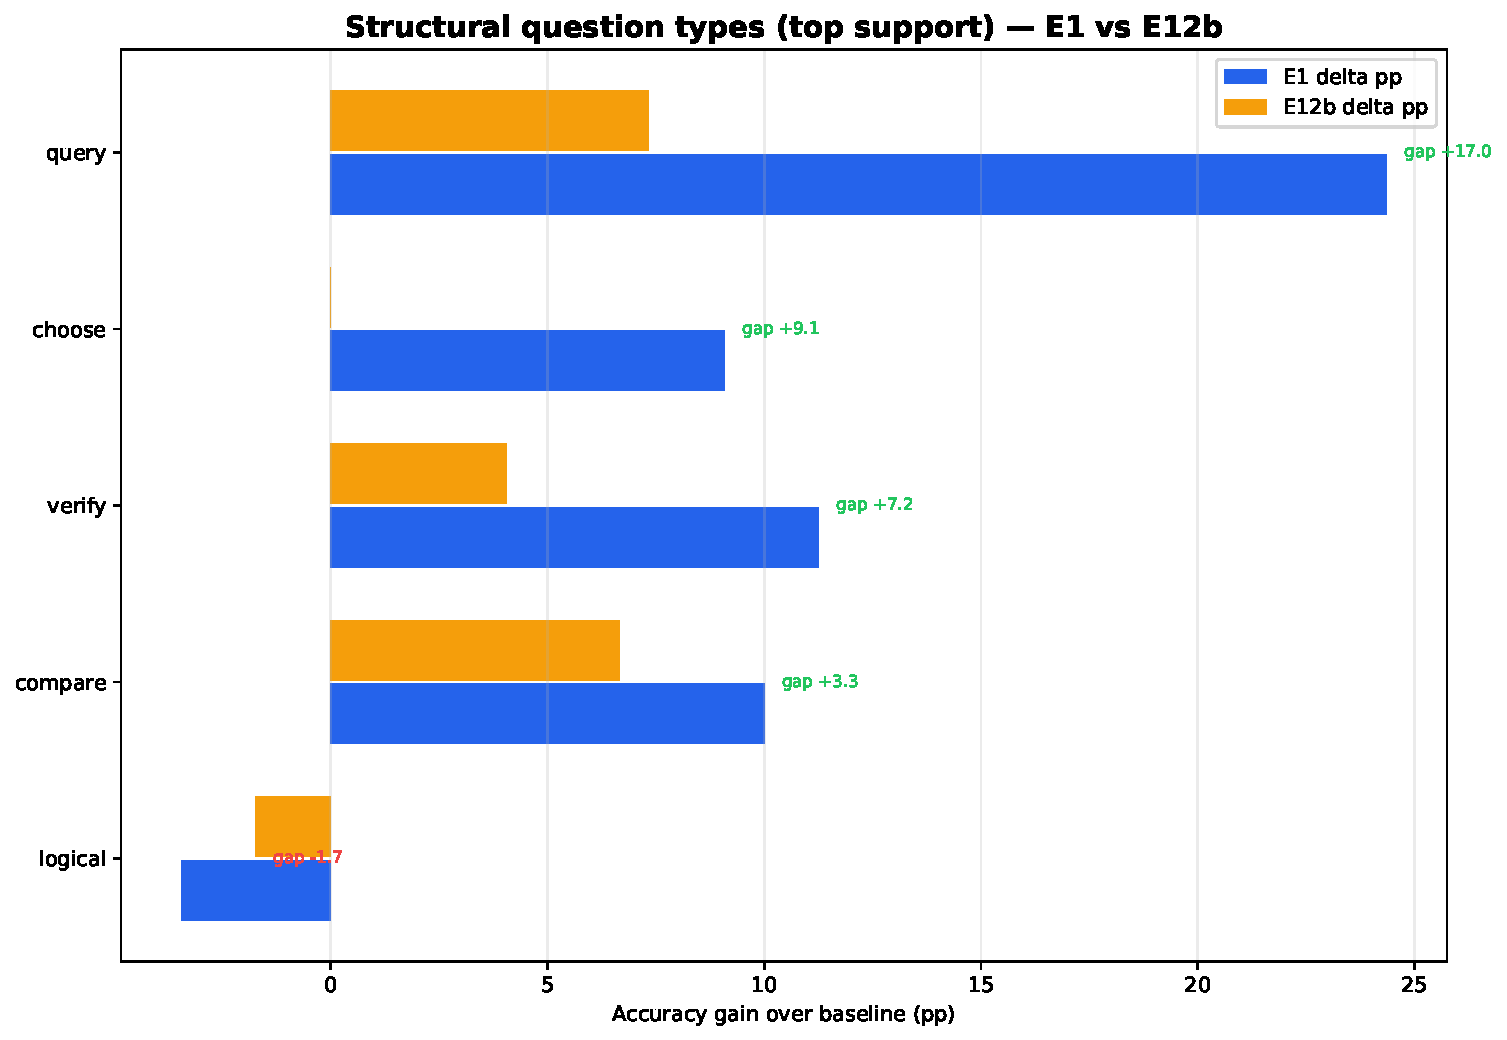
\includegraphics[width=\linewidth]{figures/task4_error_stratification_report_p2}
  \caption{Accuracy gain (pp) by structural question type for E1 (blue) and
  E12b (orange) at $n{=}500$. E1 substantially outperforms E12b for
  query-type questions (+17.0~pp gap) and choose-type (+9.1~pp gap).
  Logical questions show a slight negative for both, reflecting the low
  sample count ($n{=}116$) and high baseline accuracy.}
  \label{fig:stratified_structural}
\end{figure}

\begin{figure}[t]
  \centering
  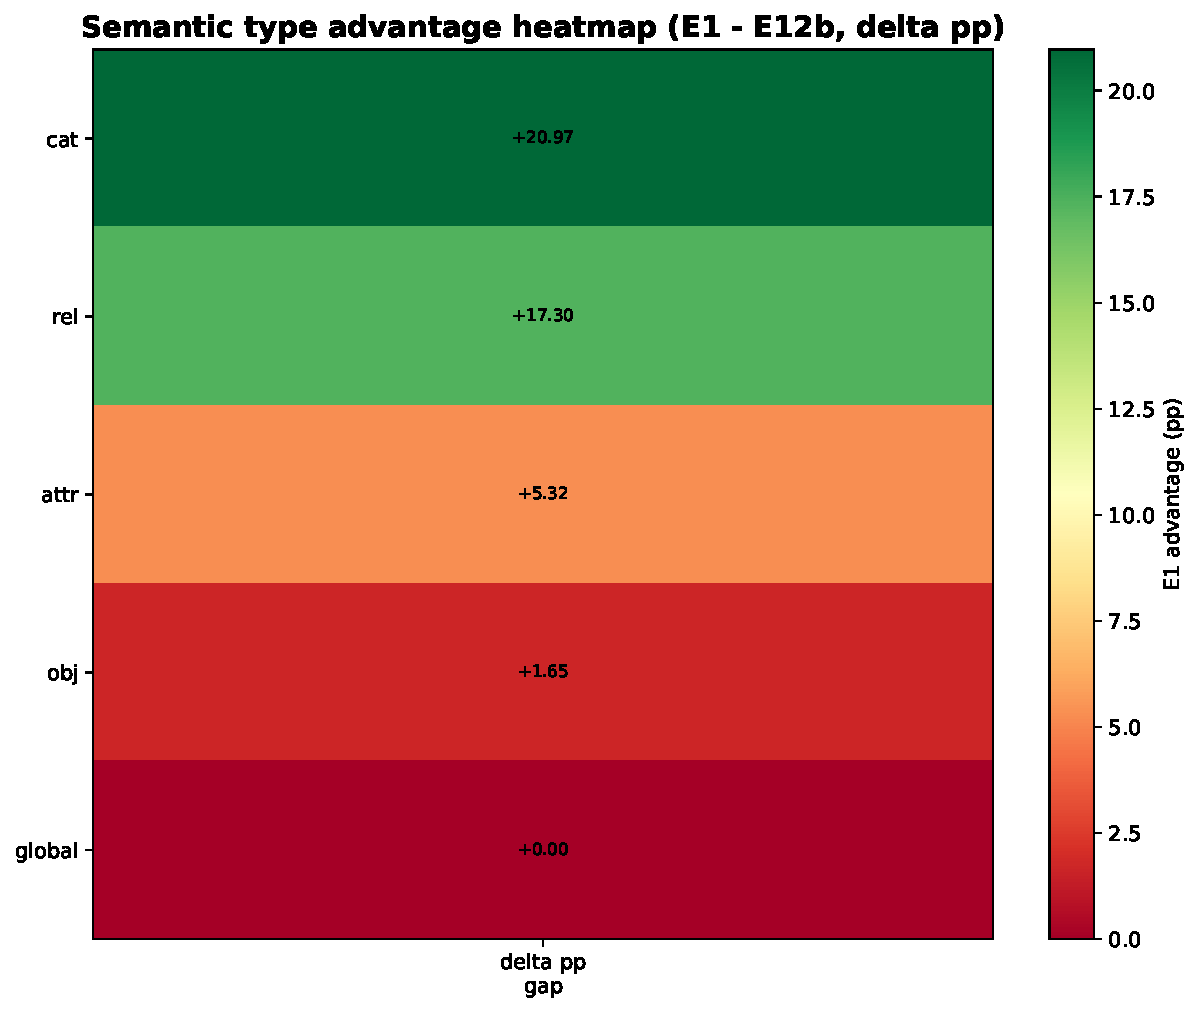
\includegraphics[width=\linewidth]{figures/task4_error_stratification_report_p3}
  \caption{E1 advantage over E12b ($\Delta$pp) by semantic question sub-type
  (heatmap). Categorical (cat: $+20.97$~pp) and relational (rel: $+17.30$~pp)
  sub-types show the strongest E1 advantage, consistent with object-existence
  and spatial claims being the most verifiable claim families.}
  \label{fig:stratified_semantic}
\end{figure}

\subsection{Targeted vs.\ Random Correction}
\label{sec:random_ablation}

To confirm that gains are claim-specific and not a consequence of generic belief
perturbation, we run a \emph{random ablation} control that removes beliefs at random
using the same budget as targeted correction. As shown in \cref{fig:random_vs_targeted},
the random flip rate is 25.0\% vs.\
60.3\% for targeted correction---a gap of $+35.3$~pp. This rules out the hypothesis
that any belief modification improves VLM answers, and confirms that the mechanism
is grounded in accurate identification and replacement of false premises.


\begin{figure}[t]
  \centering
  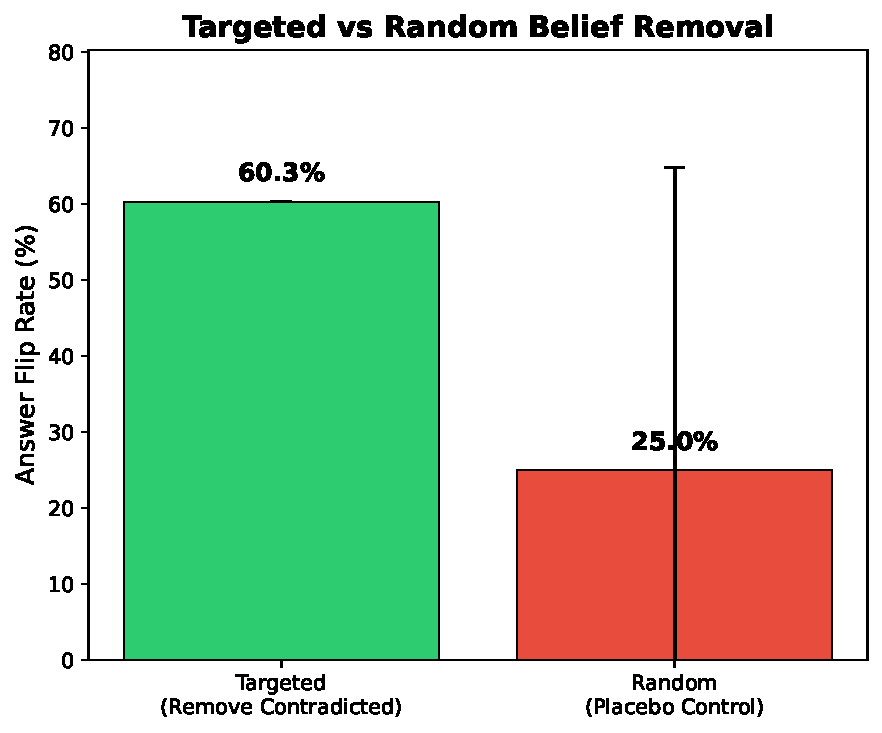
\includegraphics[width=0.75\linewidth]{figures/random_vs_targeted}
  \caption{Targeted vs.\ random belief removal on premise-error cases.
  Targeted correction (remove only contradicted beliefs) achieves a 60.3\%
  flip-to-correct rate versus 25.0\% for random removal at matched budget,
  a gap of $+35.3$~pp confirming that the intervention is claim-specific
  and not a generic perturbation effect.}
  \label{fig:random_vs_targeted}
\end{figure}

\subsection{Competitor Matrix}
\label{sec:competitor}

\Cref{tab:competitor} ranks all methods on GQA ($n{=}500$) under identical model and
data conditions. BCI-E1 leads by a margin of $+16.6$~pp over the next-best
method (Resample-Lite at 60.6\%). Self-Correct underperforms Vanilla by $10.0$~pp,
consistent with prior findings that naive self-revision can introduce
errors~\cite{huang2023large}. CoVe-Lite also underperforms Vanilla, confirming
that \bci{}'s advantage over CoVe-Lite is not attributable to the verification
step alone but to the explicit premise-replacement mechanism.

\begin{table}[h]
\centering
\caption{Full competitor matrix (GQA, $n{=}500$, Qwen2.5-VL-7B-Instruct).
All methods share the same model and question split.}
\label{tab:competitor}
\small
\begin{tabular}{lcc}
\toprule
\textbf{Method} & \textbf{Accuracy} & \textbf{Rank} \\
\midrule
BCI-E1        & 77.2\% (386/500) & 1 \\
Resample-Lite & 60.6\% (303/500) & 2 \\
Vanilla       & 59.2\% (296/500) & 3 \\
BCI-E3        & 58.6\% (293/500) & 4 \\
CoVe-Lite     & 57.2\% (286/500) & 5 \\
Self-Correct  & 49.2\% (246/500) & 6 \\
\bottomrule
\end{tabular}
\end{table}

\subsection{Statistical Significance}
\label{sec:stats}

\Cref{tab:significance} reports a condensed summary of pairwise McNemar exact
$p$-values across methods.
All key comparisons involving E1 are significant at $p{<}10^{-13}$ at $n{=}500$
and $p{<}10^{-47}$ at $n{=}2000$. E12b reaches significance at $n{=}2000$
($p{=}1.34{\times}10^{-5}$, Holm-corrected). The significance of BCI-E1 vs.\ E12b
($p{=}9.99{\times}10^{-43}$) confirms that the two policies represent meaningfully
different operating points on the accuracy/compute trade-off. BCI-E3 is not
significant ($p{=}0.84$), providing a clean negative control.

\begin{table}[h]
\centering
\caption{Pairwise McNemar exact $p$-values. BCI-E1 is highly significant at all
scales; E12b is significant at $n{=}2000$; E3 is not significant (negative control).}
\label{tab:significance}
\small
\setlength{\tabcolsep}{4pt}
\begin{tabular}{llrl}
\toprule
\textbf{Comparison} & $n$ & $p$\textbf{-value} & \textbf{Sig.?} \\
\midrule
Baseline vs.\ BCI-E1  & 500  & $1.49{\times}10^{-14}$ & \checkmark \\
Baseline vs.\ BCI-E3  & 500  & $0.839$                 & $\times$   \\
Baseline vs.\ BCI-E1  & 2000 & $1.78{\times}10^{-48}$  & \checkmark \\
Baseline vs.\ E12b    & 2000 & $1.34{\times}10^{-5}$   & \checkmark \\
BCI-E1 vs.\ E12b      & 2000 & $9.99{\times}10^{-43}$  & \checkmark \\
\bottomrule
\end{tabular}
\end{table}

\Cref{fig:sig_n500,fig:sig_n2000} show the full pairwise significance tables
at $n{=}500$ (all 56 method pairs across 6 methods) and the $n{=}2000$ subset.
The complete matrix confirms that BCI-E1 wins every pairwise comparison at
$p{<}10^{-10}$ at $n{=}500$, and that E12b is a statistically robust
improvement over Vanilla at both scales while remaining significantly below E1.

\begin{figure}[t]
  \centering
  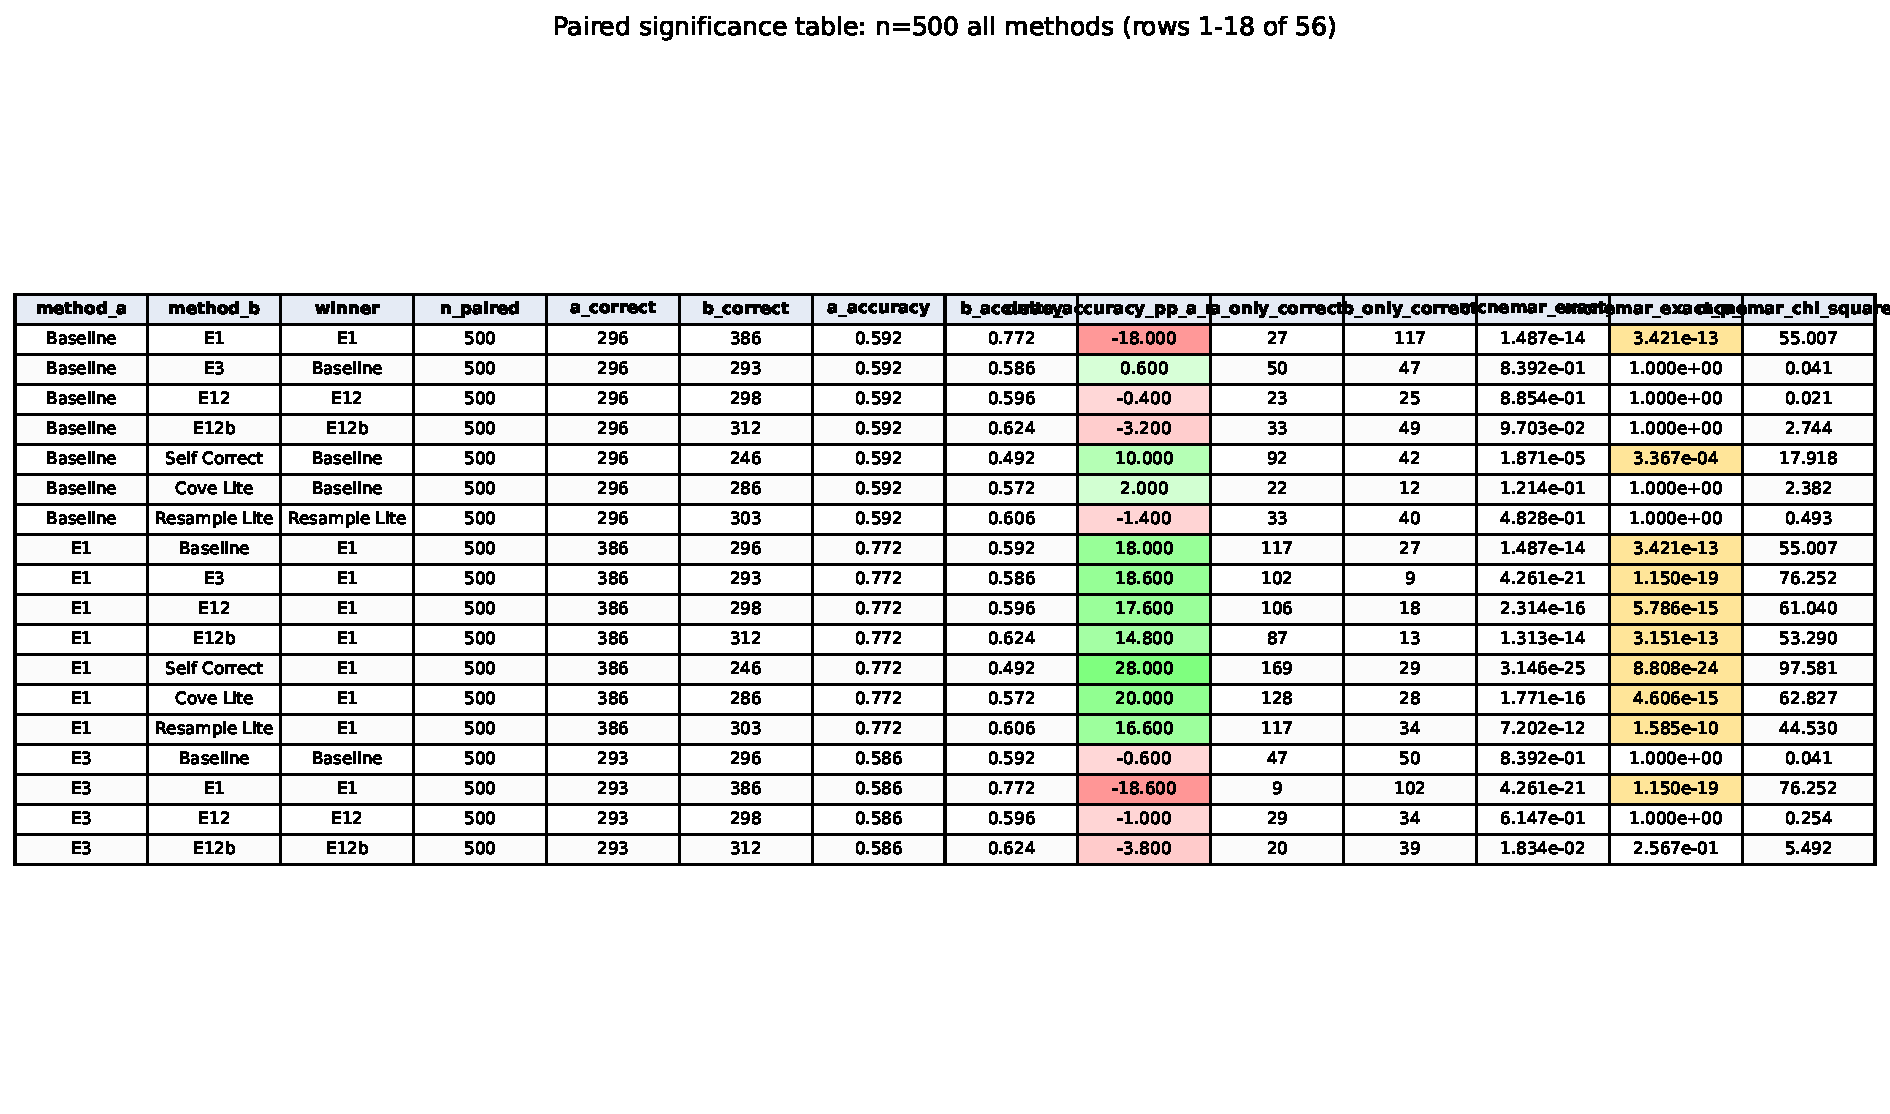
\includegraphics[width=\linewidth]{figures/paired_significance_tables_p1}
  \vspace{1pt}
  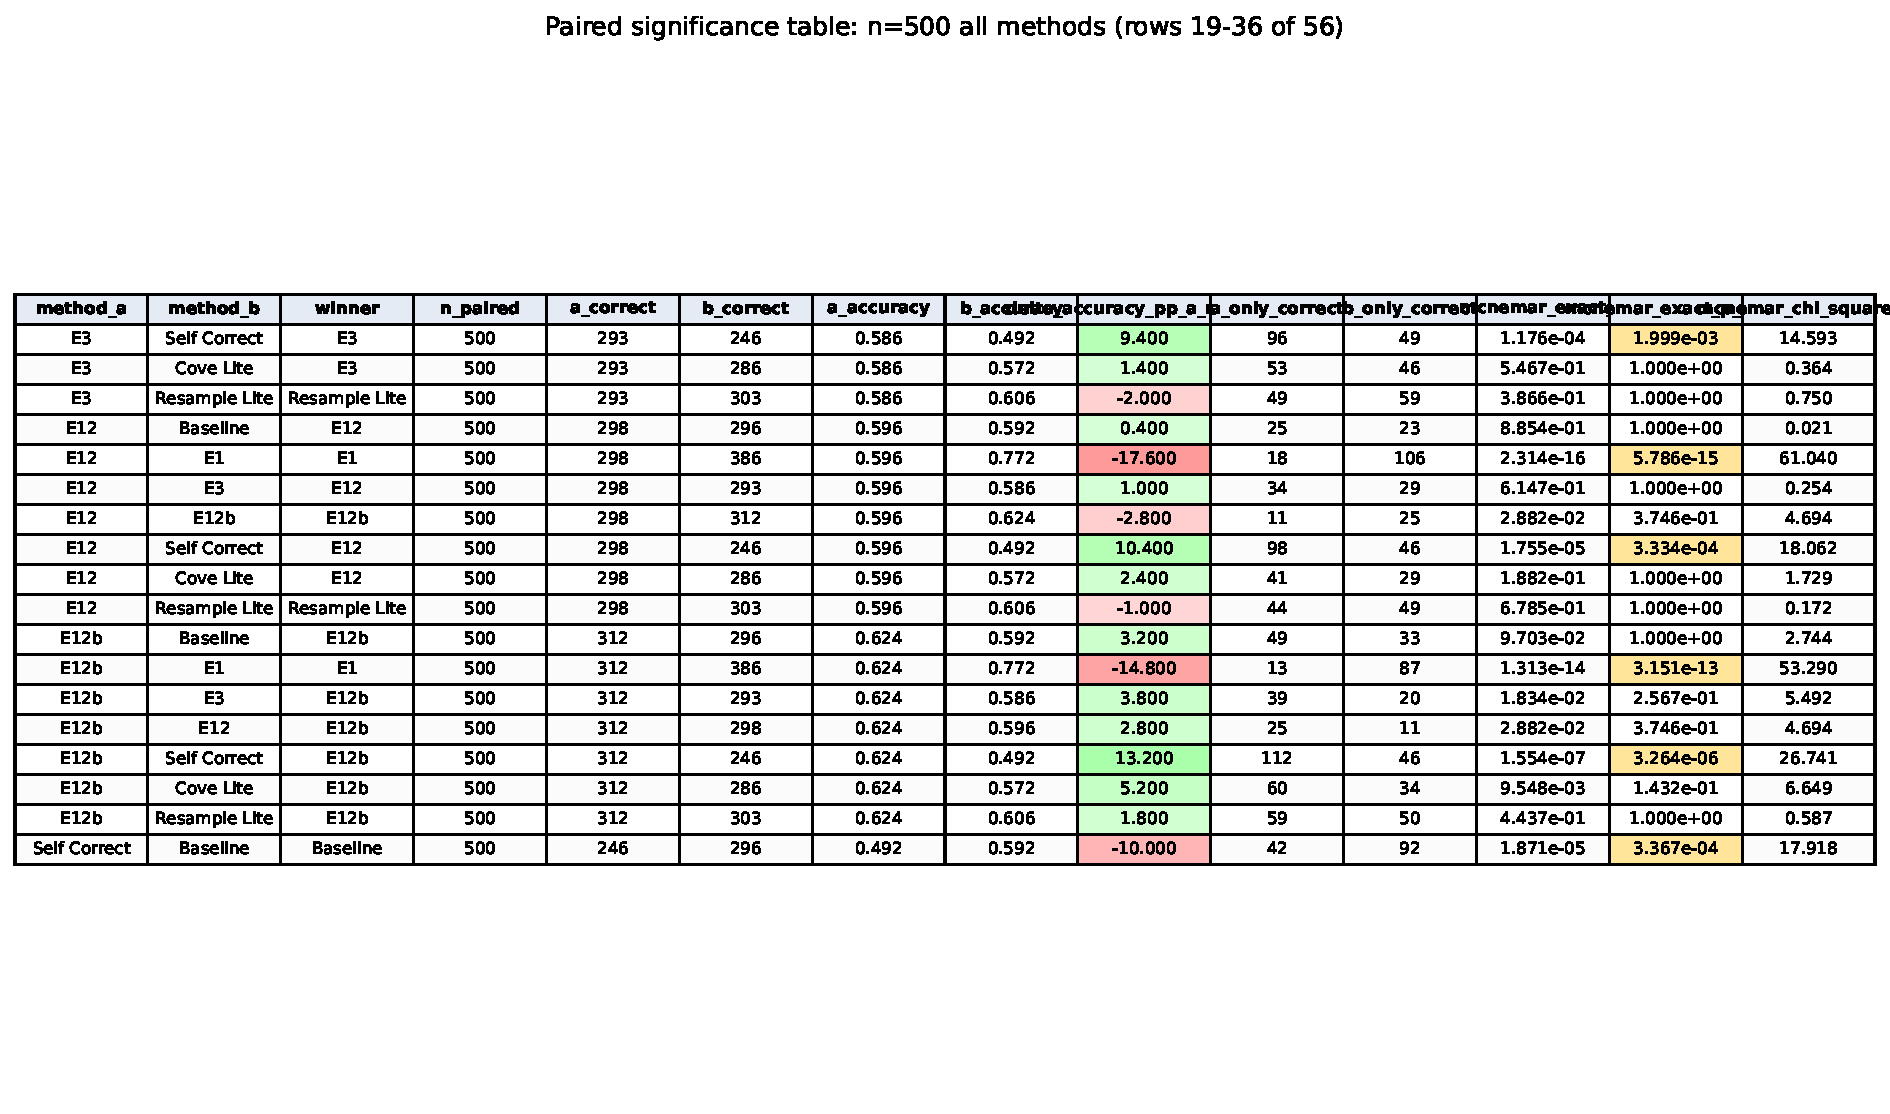
\includegraphics[width=\linewidth]{figures/paired_significance_tables_p2}
  \vspace{1pt}
  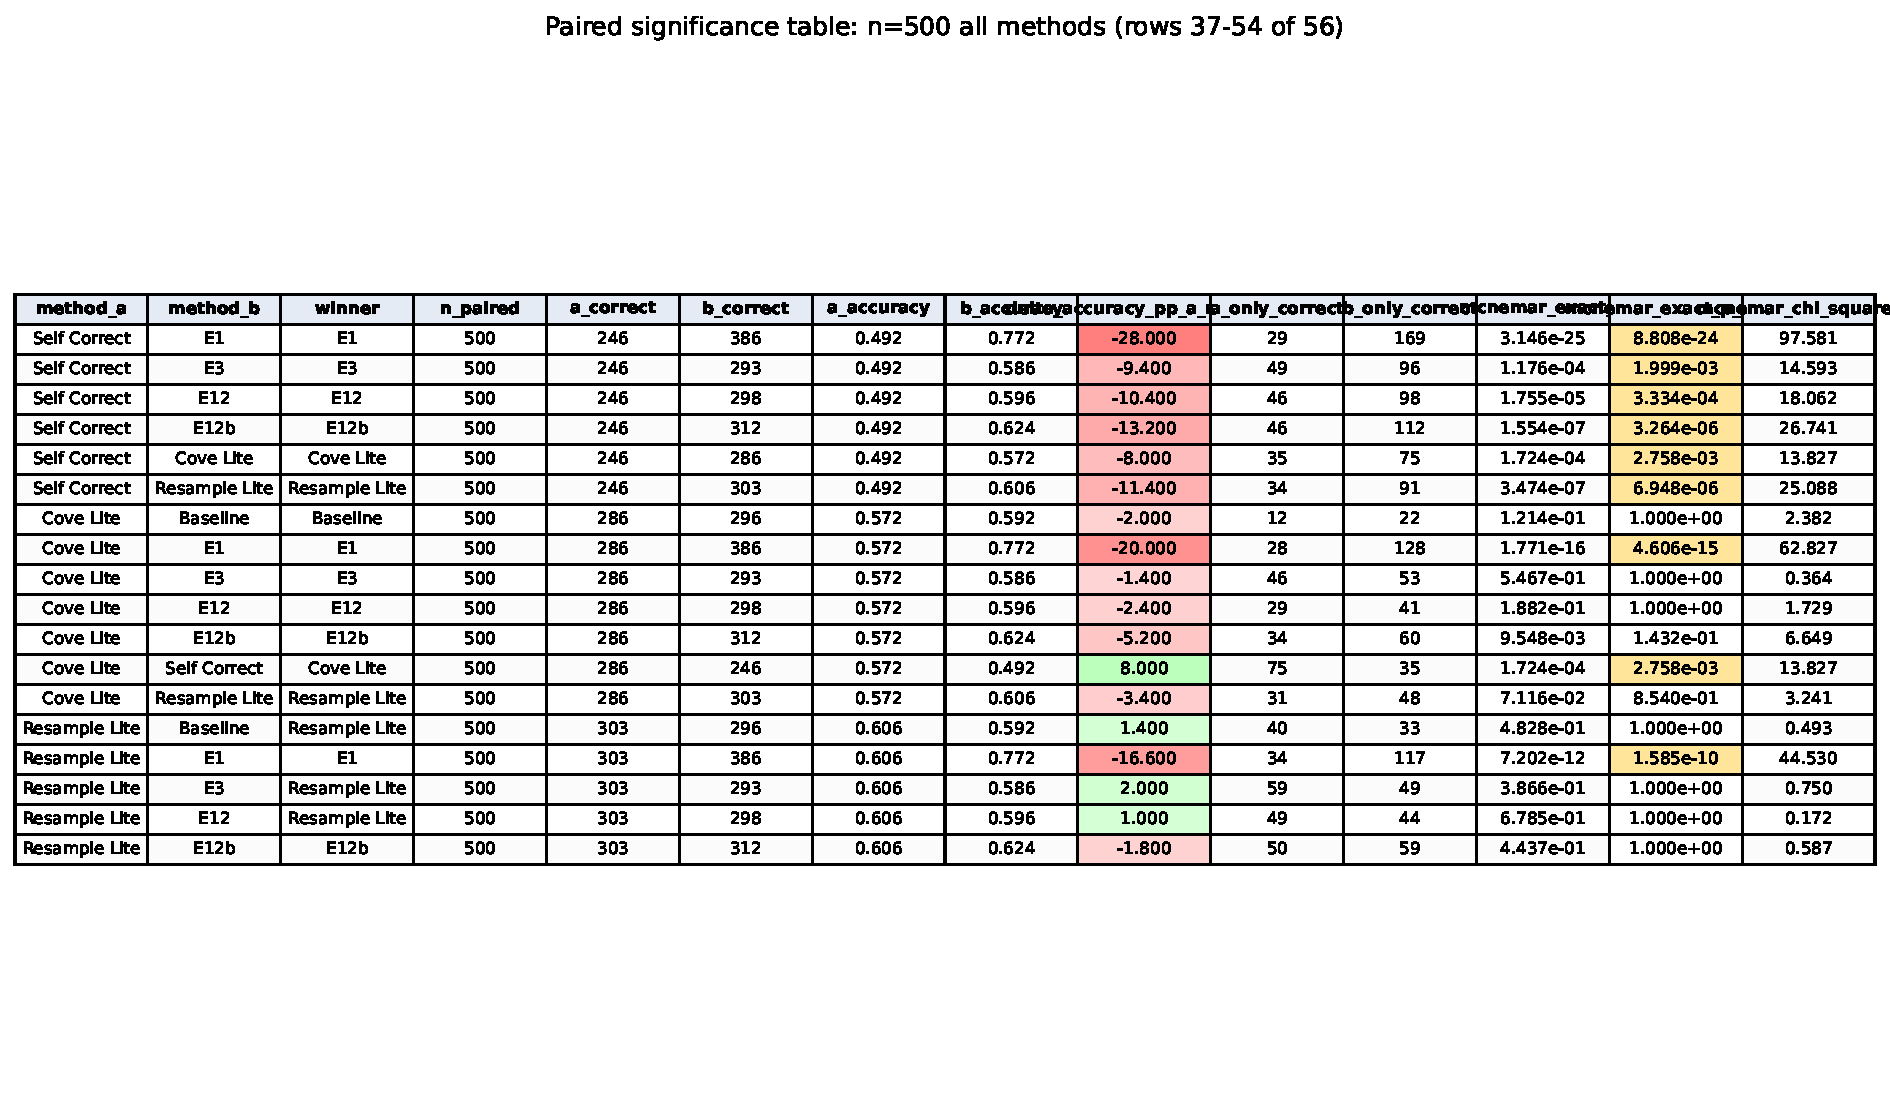
\includegraphics[width=\linewidth]{figures/paired_significance_tables_p3}
  \vspace{1pt}
  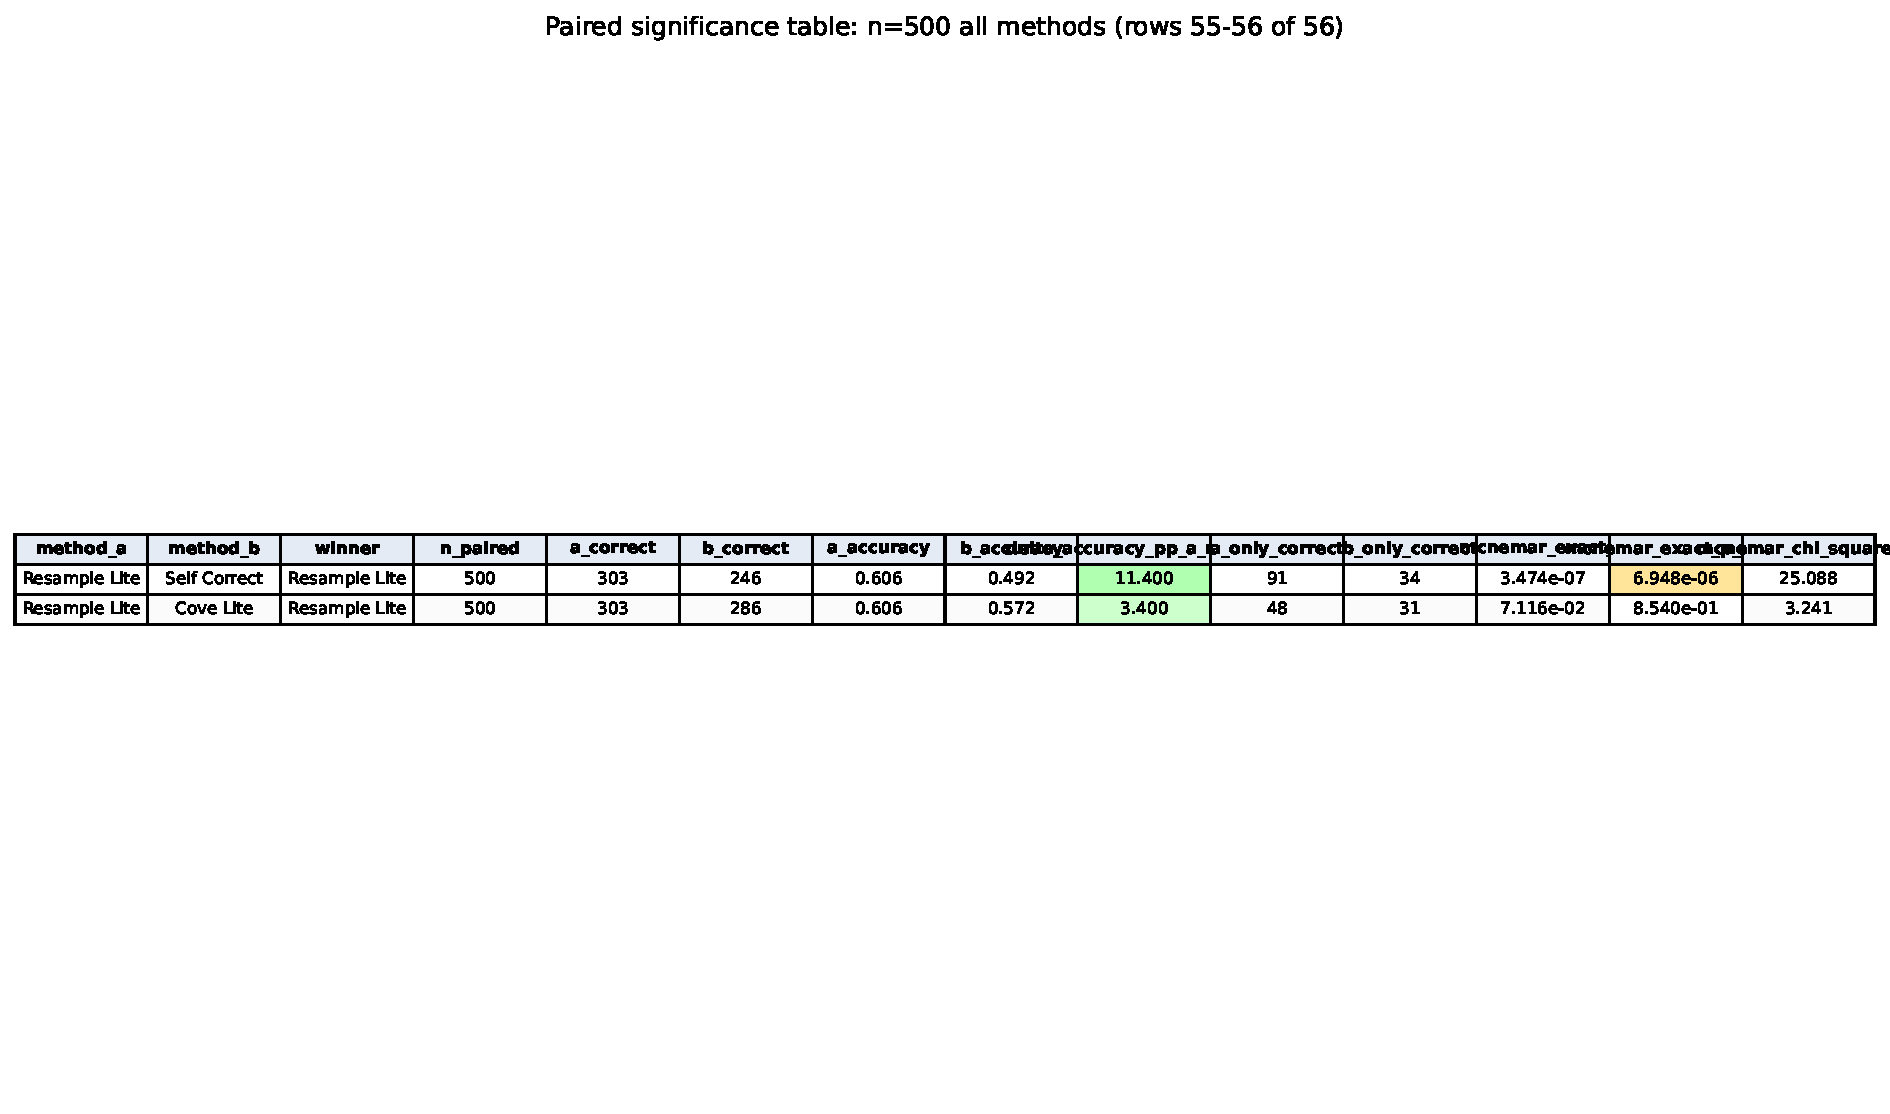
\includegraphics[width=\linewidth]{figures/paired_significance_tables_p4}
  \caption{Full pairwise McNemar significance table at $n{=}500$ (all 56 pairs
  across 6 methods: Baseline, E1, E3, E12, E12b, Self-Correct, CoVe-Lite,
  Resample-Lite). Cells highlighted green/red indicate significant wins/losses;
  yellow indicates marginal significance. BCI-E1 wins every comparison
  at $p{<}10^{-10}$.}
  \label{fig:sig_n500}
\end{figure}

\begin{figure}[t]
  \centering
  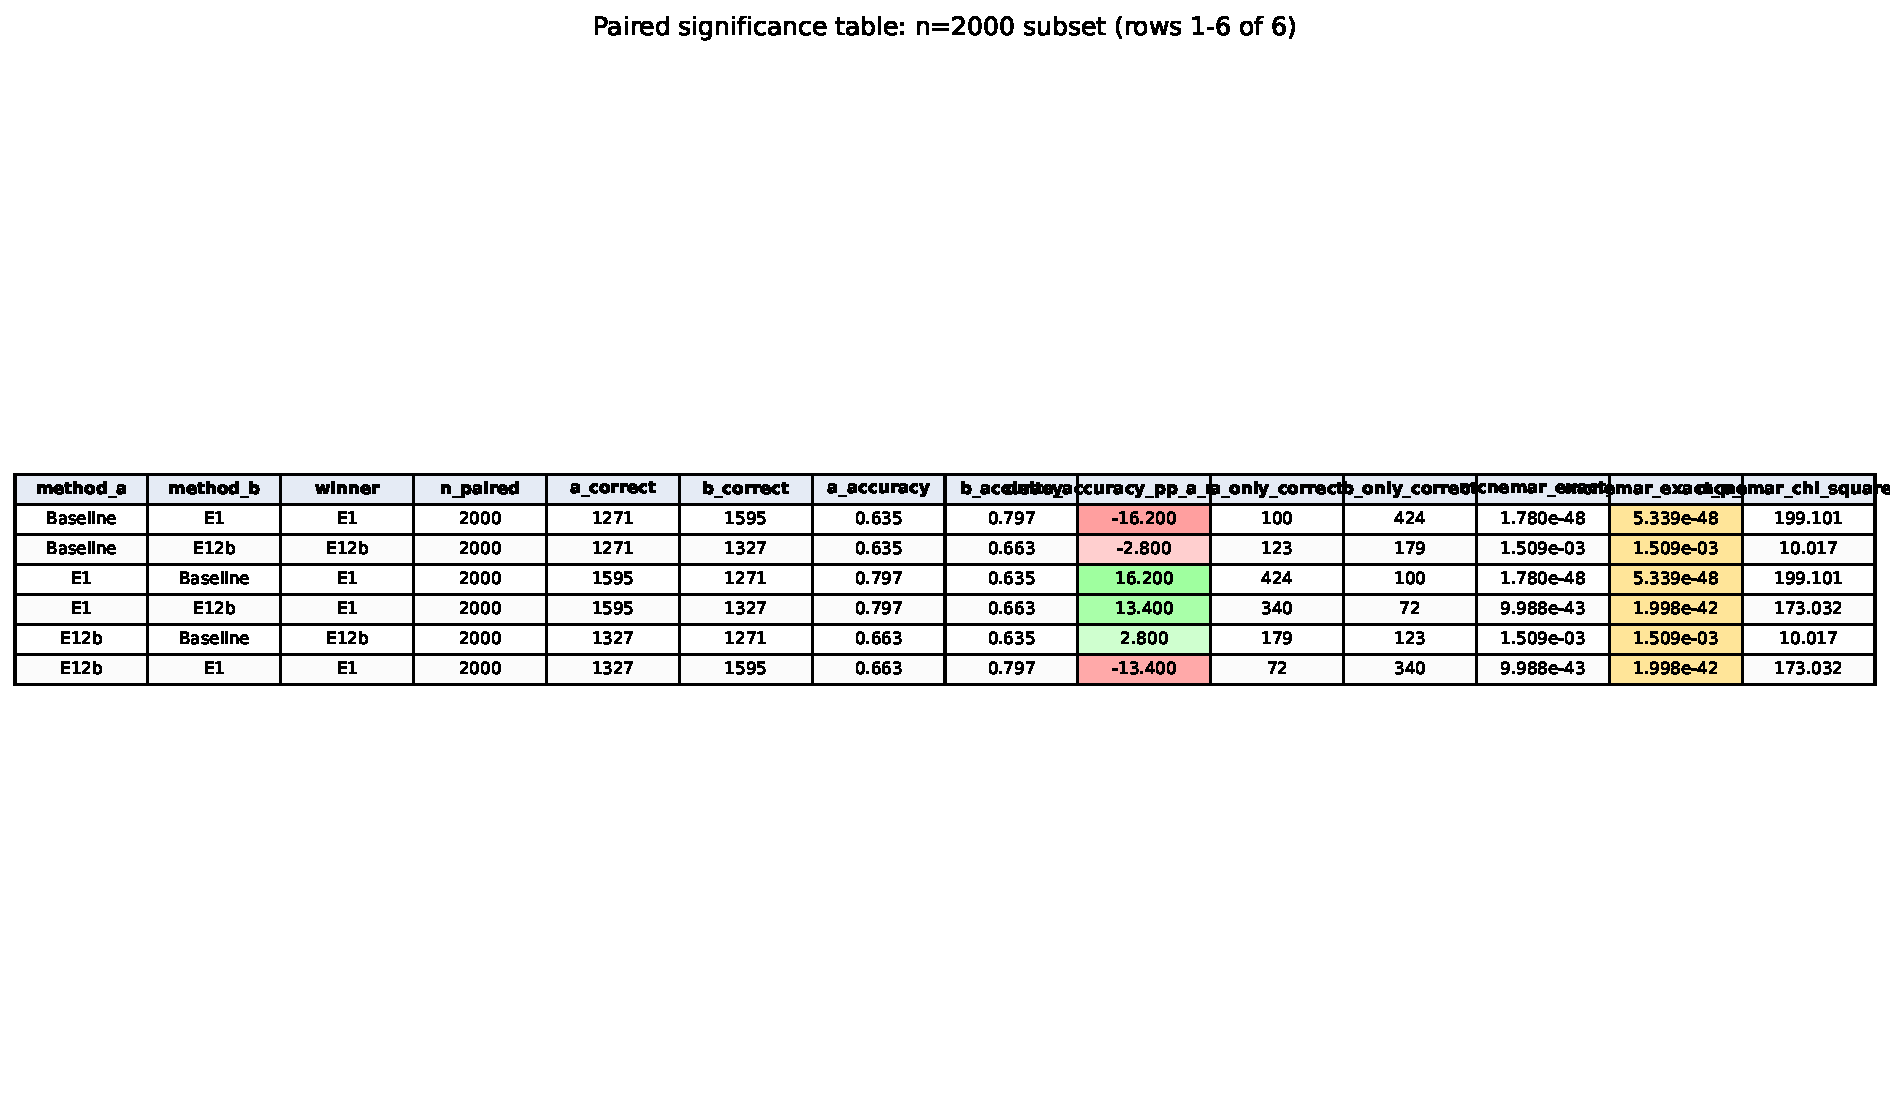
\includegraphics[width=\linewidth]{figures/paired_significance_tables_p5}
  \caption{Pairwise McNemar significance at $n{=}2000$ (Baseline, E1, E12b).
  E1 vs.\ Baseline: $p{=}1.78{\times}10^{-48}$;
  E12b vs.\ Baseline: $p{=}1.51{\times}10^{-3}$ (Holm-corrected);
  E1 vs.\ E12b: $p{=}9.99{\times}10^{-43}$.}
  \label{fig:sig_n2000}
\end{figure}

\subsection{Cross-Benchmark Generalization (POPE)}
\label{sec:pope}

To assess whether \bci{} generalizes beyond GQA, we evaluate \textbf{BCI-E12b}
on \textbf{POPE}~\cite{li2023evaluating}, a hallucination benchmark with three
adversarially-stratified splits (Adversarial, Popular, Random), each $n{=}500$.
POPE uses binary yes/no questions about object existence, making it structurally
distinct from GQA's compositional reasoning questions.

\Cref{fig:pope_results} shows that BCI-E12b yields consistent positive gains
across all three splits: $+2.2$~pp on Adversarial ($83.4\% \to 85.6\%$;
26 flips), $+2.4$~pp on Popular ($83.4\% \to 85.8\%$; 27 flips), and
$+1.8$~pp on Random ($85.2\% \to 87.0\%$; 21 flips). All gains are positive
despite POPE's high baseline accuracy ($>83\%$), confirming that BCI-E12b
can improve results even in near-ceiling regimes.

\Cref{fig:pope_cross_benchmark} places these gains in context alongside GQA.
The POPE gains ($+1.8$--$+2.4$~pp) are smaller than GQA ($+2.8$~pp at
$n{=}2000$) but structurally consistent: \bci{} improves accuracy on every
benchmark tested, confirming that premise-error correction is not a
GQA-specific artifact.

\begin{figure}[t]
  \centering
  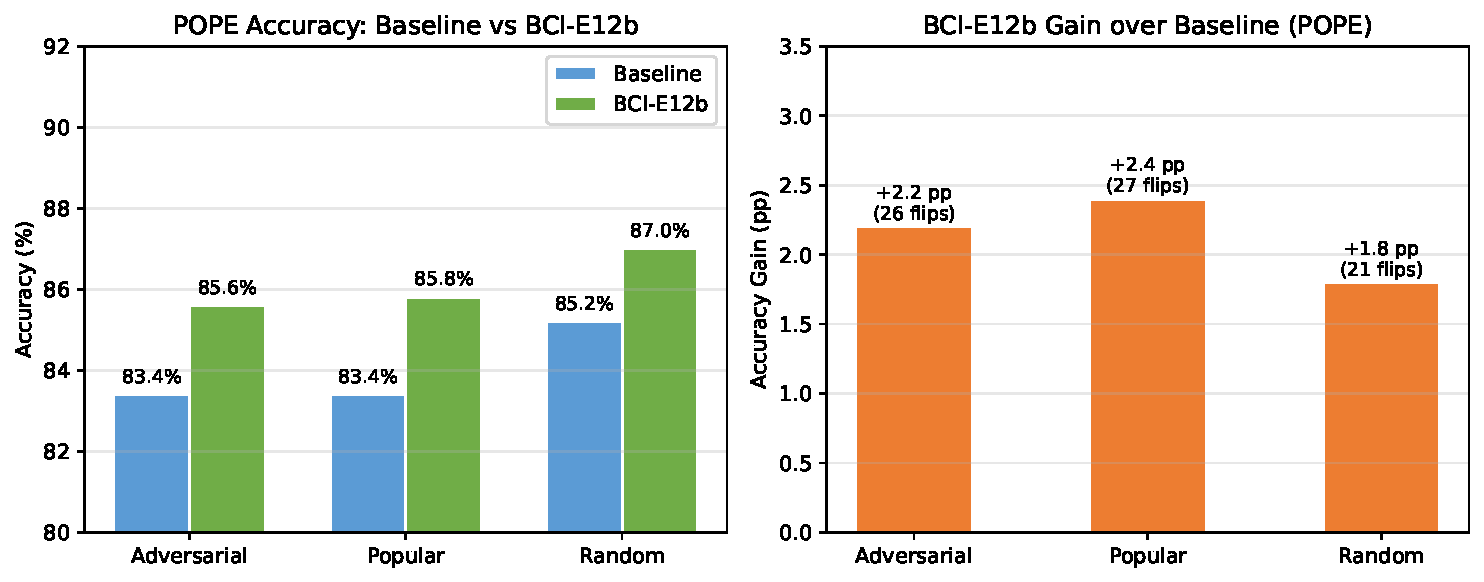
\includegraphics[width=\linewidth]{figures/pope_results}
  \caption{BCI-E12b results on POPE ($n{=}500$ per split).
  Left: baseline vs.\ corrected accuracy per split. Right: accuracy gain (pp)
  and flip count. BCI-E12b yields $+1.8$--$+2.4$~pp across all three
  adversarial splits, demonstrating positive generalization to a structurally
  different hallucination benchmark.}
  \label{fig:pope_results}
\end{figure}

\begin{figure}[t]
  \centering
  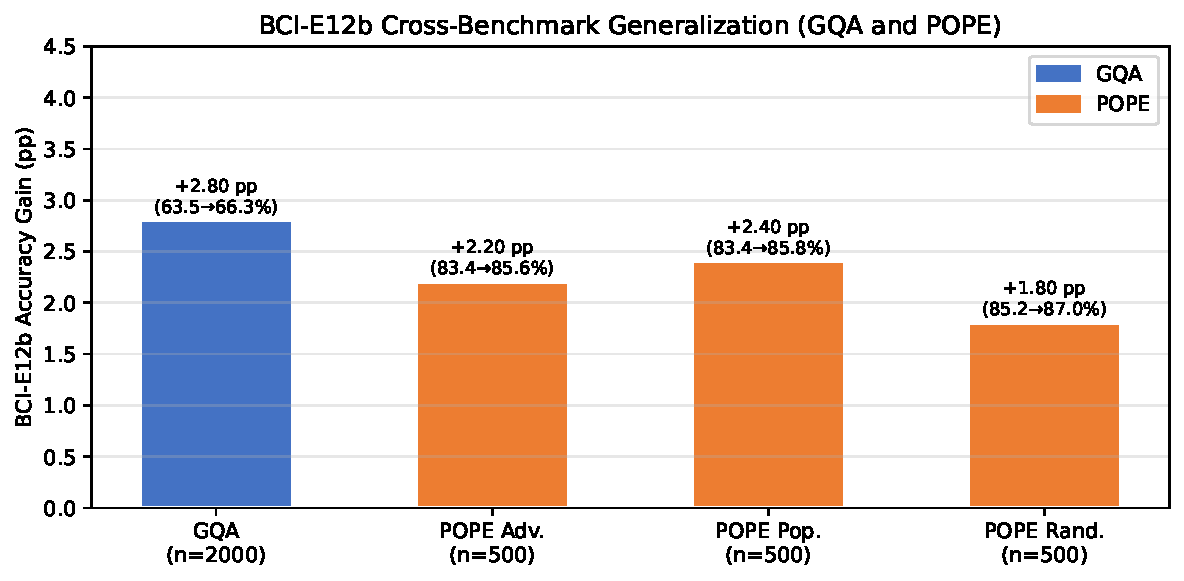
\includegraphics[width=\linewidth]{figures/pope_cross_benchmark}
  \caption{BCI-E12b cross-benchmark accuracy gain (pp) on GQA and all three
  POPE splits. Gains are positive and consistent across benchmarks ($+1.8$--$+2.8$~pp),
  confirming that premise correction generalizes beyond the GQA evaluation setting.}
  \label{fig:pope_cross_benchmark}
\end{figure}
